\chapter{Konzept}\label{konzept}
\section{Allgemein}
\subsection{Ausgangslage}
Als Rich Client Framework wird Eclipse 3.x\footnote{die aktuelle Version ist 3.7 (stand: 31.8.2011)} genommen. Siehe Abschnitt \titleref{selection_rcp_fw}. In der Folge werden die für die Eclipse Plattform gebräuchlichen Begrifflichkeiten verwendet. 

\subsection{Lizenzierung der Software}
Die Software wird lizenziert unter der Eclipse Public License\footnote{http://www.eclipse.org/legal/epl-v10.html} in der Version 1.0. Dies ist eine freie Software-Lizenz und gewährt das Recht zur freien Nutzung, Weiterverbreitung und Veränderung der Software. Die Benutzung einer Open-Source Lizenz hat insbesondere folgende Vorteile:
\begin{itemize}
	\item An der Entwicklung von Open-Source Software können sich eine beliebige Anzahl an Entwicklern beteiligen. Der Entwicklungsaufwand kann skaliert werden.
	\item Jedermann kann Erweiterungen entwickeln oder Fehler beheben.
\end{itemize}

\section{Architektur}
\subsection{Problemstellung}\label{konzept_uebersicht}
Aufgrund der Anforderung QRQ-S-01 (Erweiterbarkeit) muss die Analyse-Software auch hinsichtlich anderer Logformate erweiterbar sein. Die Applikation wird also nicht zwingendermassen mit der Erweiterung für JRockit Logdateien verwendet. Es könnte zu einem späteren Zeitpunkt sein, dass man damit Garbage Collection Logs der HotSpot Virtual Machine auswertet. Dies hat hinsichtlich Architektur einige Konsequenzen:
\begin{itemize}
	\item Die Applikation soll in zwei Komponenten aufgeteilt werden:
		\begin{itemize}
			\item Basissoftware
			\item Erweiterung JRockit
		\end{itemize}
		Die Basissoftware kann unabhängig von den Erweiterungen installiert werden, für die Auswertung einer Logdatei ist allerdings die entsprechende Erweiterung zu installieren. Eine Erweiterung kann ohne Basissoftware nicht gebraucht werden.
	\item Die Architektur der Applikation muss es zulassen, dass zu einem späteren Zeitpunkt auch Garbage Collection Logs von anderen Virtuellen Machinen analysiert werden können.
	\item Die Basissoftware stellt Extension-Points\footnote{Ein Extension-Point ist ein Mechanismus der von Eclipse zur Verfügung gestellt wird, damit eine Komponente (Plugin) sich bei einer anderen registrieren kann.} bereit, über welche sich die Erweiterungen  registrieren.
\end{itemize}

\subsection{Übersicht}
Die im Abschnitt \titleref{konzept_uebersicht} beschriebenen Konsequenzen führen dazu, dass die Applikation - obwohl es momentan erst die Erweiterung für die JRockit Garbage Collection Logs gibt - in zwei verschiedene Features aufgeteilt wird. Die beschriebenen Anforderungen können grob folgendermassen zugewiesen werden:
\begin{itemize}
	\item Basissoftware (Core Feature)
		\begin{itemize}
			\item Garbage Collection Log importieren
			\item Garbage Collection Log einlesen
			\item Profil erstellen, speichern, exportieren, importieren
			\item Hilfesystem
		\end{itemize}
	\item JRockit Extension (JRockit Extension Feature)
		\begin{itemize}
			\item Garbage Collection Log parsen
			\item Standardauswertung: Heap, Dauer Garbage Collection
		\end{itemize}
\end{itemize}

\subsection{Projektstruktur}\label{projektstruktur}
Wie im Abschnitt \titleref{installation} erläutert, besteht die Software aus zwei getrennten Features. Das Core-Feature ist die Basis und verantwortlich für den gesamten Import-Prozess (Import-Wizard, Leseprozess der Log-Datei, Anzeige der Menus, Profil-Verwaltung, etc.). Die JRockit Extension ist eine für die Garbage Collection Logs der JRockit geschriebene Erweiterung. Sie ist für das Parsing der Logdateien, die Aufbereitung und Bereitstellung der Daten zuständig. Beinhaltet aber keine Basisfunktionalität.
 \begin{figure}[H]
  	\centering
    	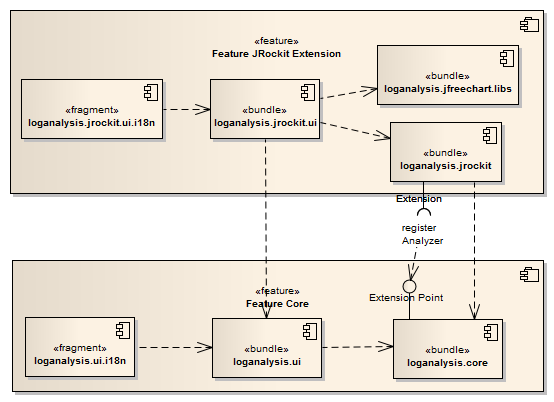
\includegraphics[width=14cm]{images/architektur_komponenten_uebersicht}
        	\caption{Architektur: Komponentendiagramm}
\end{figure}

Das Core Feature besteht aus dem Modul User Interface (``loganalysis.core.ui'') und einem von JFace und SWT\footnote{JFace und SWT wird in Eclipse als Library für die Präsentationsschicht verwendet.} unabhängigen Teil (``loganalysis.core''). Öffnet der Benutzer eine Garbage Collection Logdatei, wird diese durch das Core Feature eingelesen und an alle verfügbaren Extensions weitergeleitet. Die erste Extension welche den Inhalt der Datei versteht, öffnet seine dafür vorgesehenen Reports und Charts. Jede Extension hat ein basierend auf der Logdatei eigenes Domänen-Modell.

\subsubsection{Weitere Projekte}
Einige Plugins wurden im vorherigen Abschnitt nicht erwähnt:
\begin{itemize}
	\item Test-Projekte\footnote{Der Test-Code befindet sich in eigenen Projekten (siehe Abschnit \ref{testing}).}
		\begin{itemize}
			\item core.test
			\item core.ui.test
			\item jrockit.test
			\item jrockit.ui.test
		\end{itemize}
	\item  Features\footnote{Features sind in sich lauffähige Softwarekomponenten mit definiertem Umfang.}
		\begin{itemize}
			\item loganalysis.feature
			\item loganalysis.jrockit.feature
		\end{itemize}
	\item  Thirdparty Bibliotheken\footnote{Thirdparty Bibliotheken werden bei Eclipse-Anwendungen als Plugins gepackt.}
		\begin{itemize}
			\item  loganalysis.jfreechart.libs (JFreeChart Library)
		\end{itemize}
	\item  Targetplattform\footnote{Definiert gegen welche Plattform die Anwendung entwickelt wird.}
		\begin{itemize}
			\item  loganalysis.targetplatform (beinhaltet die Target-Plattform)
		\end{itemize}
	\item  Update-Seite\footnote{Definiert bereitgestellte Features}
		\begin{itemize}
			\item loganalysis.updatesite (definiert und generiert die Update-Seite)
		\end{itemize}
\end{itemize}

\subsection{Ablauf Garbage Collection Analyse}
Beim öffnen einer Analyse wird die zuständige Extension gesucht\footnote{Extensions registrieren sich via das plugins.xml an einem Extension-Point. }, welche den Inhalt\footnote{Der Inhalt der Datei wird lazy via die Methode getContent und einem ContentReader geladen.} der Logdatei versteht. Die Erweiterung ist für das Parsen und Aufbereiten der Daten und die Anzeige in einem Analysefenster zuständig. 
 \begin{figure}[H]
  	\centering
    	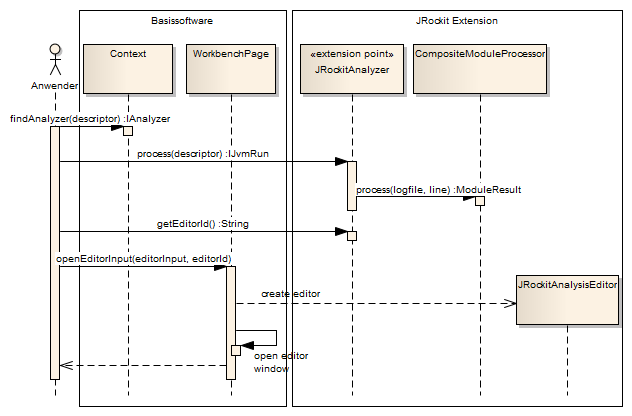
\includegraphics[width=16cm]{images/core_sequence_analysis}
	\caption{Sequenz-Diagramm Öffnen der Analyse}
\end{figure}
Der Ablauf der Garbage Collection Analyse ist folgendermassen:
\begin{enumerate}
	\item Via Context wird die Erweiterung\footnote{Erweiterungen registrieren sich als Extensions an Extension-Points. Diese Konfiguration befindet sich im plugin.xml.} gesucht.
	\item Analyzer der Erweiterung parst inhalt und gibt ihn als Objekt zurück.
	\item Editor wird geöffnet, das Objekt wird als Input übergeben.
\end{enumerate}

\section{Basissoftware}
\subsection{Installation (FRQ-01)}\label{installation}
Zur Installation der Software benötigt man die Eclipse-Entwicklungsumgebung in der Version 3.7. Darin integriert befindet sich ein Update-Manager, der Software-Komponenten von Lokal oder dem Netzwerk installieren kann. Auch Updates werden über diesen Mechanismus installiert. Die Analyse-Software wird via eine Update-Seite bereitgestellt. Der Software-Build durch das Continuous Integration System publiziert die Artefakte (Features, Plugins) auf einen via Internet zugänglichen Server, von welchem der Update-Manager die Software herunterlädt um anschliessend zu importieren. Update-Seiten im Eclipse-Umfeld bestehen aus Features (Eclipse Feature-Projekt). Features bestehen aus unterschiedlichen Plugins (Eclipse Plugin-Projekt). Eclipse\footnote{in der Basis ist es Equinox, die Implementation des OSGi Standards} ist in der Lage, Plugins zur Laufzeit zu installieren, starten, deinstallieren.

Die Update-Seite für diese Software wird folgendermassen aufgebaut:
\begin{itemize}
\item \textbf{Basissoftware:} Umfasst alle Plugins , die für die Basissoftware notwendig sind. Siehe Abschnitt \titleref{projektstruktur}.
\item \textbf{JRockit Erweiterung: }Umfasst alle Plugins zur JRockit Erweiterung und hat zugleich die \textbf{Abhängigkeit auf das Basissoftware-Feature}.
\end{itemize}

\subsection{Update (FRQ-02)}
Der Update eines Features auf der Update-Seite ist erkennbar durch eine Änderung der Major respektive Minor Version oder aber durch Änderung des an die Feature-Datei angehängten Zeitstempels\footnote{Mittels der Versionnummer x.x.qualifier erreicht man, dass der Zeitstempel ans Dateiende gehängt wird.}. Beim Starten der Software wird überprüft, ob ein sich auf dem Server befindendes Feature aktualisiert wurde. Der Benutzer kann diese im laufenden Betrieb der Applikation installieren. Danach ist allerdings ein Neustart der Applikation nötig. 

\subsection{Datei importieren (FRQ-03)}
Der Import einer Logdatei findet über einen Import-Wizard statt. Der Ablauf zum Import einer oder mehrerer Dateien ist folgendermassen:
\begin{enumerate}
	\item Import-Wizard öffnen
	\item Auswahl des Ordners
	\item Selektion einer oder mehrerer Logdateien
	\item Bestätigung der Eingaben
	\item Anschliessend wird die Logdatei als Instanz von IFileDescriptor in der Ansicht Logdateien angezeigt.
\end{enumerate}

\subsubsection{Importierte Dateien speichern (FRQ-03.1)}
Der im Abschnitt \ref{memento} beschriebene Mechanismus wird verwendet, damit nach einem Neustart der Entwicklungsumgebung die importierten Logdateien nicht verloren gehen. 

\subsection{Datei einlesen (FRQ-04)}
Durch den Import einer Garbage Collection Datei erscheinen diese im Logdateien-Fenster. Das öffnen einer dieser Dateien lädt den Inhalt in den Arbeitsspeicher. Die Daten sind noch unstrukturiert und werden innerhalb des im nächsten Abschnitt definierten Domänenmodells gespeichert.

\subsubsection{Domänenmodell}
\textit{IFileDescriptor} wird für die Abstraktion der Garbage Collection Logdatei verwendet. Darin enthalten sind Metadaten wie Dateiname und Pfad sowie - wenn bereits geladen - der Inhalt der Datei. Die Abstraktion einer Garbage Collection Logdatei heisst \textit{AbstractJvmRun} und wird erst von der jeweiligen Erweiterung realisiert.
 \begin{figure}[H]
  	\centering
    	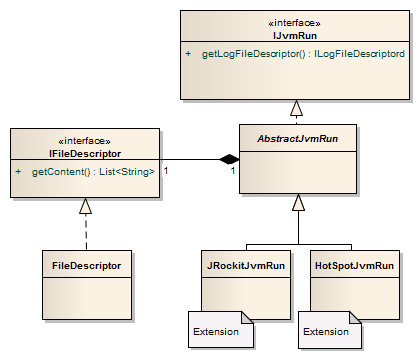
\includegraphics[width=16cm]{images/core_domain}
        	\caption{Domänenmodell: Eingelesene Datei}
\end{figure}


\subsection{Profil erstellen (FRQ-07)}
Die Ansicht Profile zeigt die vom Benutzer erstellten Profile\footnote{Initial befindet sich darin allerdings nur das Standard-Profil.}. Die Beschreibung eines Analysefensters (Name, Beschreibung, Charts mit Serien, etc.) wird anhand von Profilen definiert. Es gibt folgende zwei Arten:
\begin{itemize}
	\item \textbf{Unveränderlich Profil:} Das Standard-Profil ist aktuell das einzige unveränderliche Profil.
	\item \textbf{Veränderlich Profil:} Ein veränderliches Profil wird zur Speicherung des vom Benutzer definierten Analysefensters verwendet. Alle Änderungen die der Benutzer am Analysefenster macht (Chart hinzufügen, Chart konfigurieren), werden via ein Data-Binding an das Profil propagiert. Durch das Speichern des Profils hat der Benutzer die Möglichkeit, die selbe Analyse auch zu einem späteren Zeitpunkt an der gleichen oder einer anderen Logdatei durchzuführen.
\end{itemize}

\subsubsection{Domänenmodell}
\textit{IConfiguration} dient zur Gruppierung von profilen. Pro Extension wird eine Konfiguration mit verschiedenen Profilen abgelegt. Innerhalb eines Profils können unterschiedliche Diagramme (\textit{IChart}) angelegt werden, welche wiederum durch Achsen (\textit{IAxis}) und deren Datenquellen \textit{IValueProvider} definiert sind. \textit{IValueProvider} definieren den Weg, wie die Daten aus dem Domänenmodell gelesen werden.
 \begin{figure}[H]
  	\centering
    	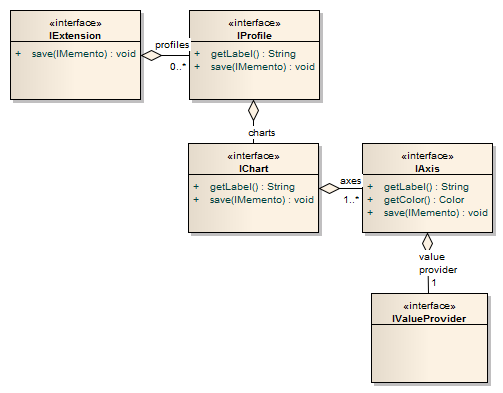
\includegraphics[width=11cm]{images/core_domain_profiles}
        	\caption{Domänenmodell: Profile}
\end{figure}

\subsubsection{Charts definieren (FRQ-07.1)}
Bei der Benutzung eines veränderlichen Profils hat der Benutzer die Möglichkeit, dem Analysefenster weitere Charts respektive Diagramme hinzuzufügen oder aber bereits existierende Diagramme zu manipulieren (weitere Serien hinzufügen, Serien entfernen, etc.). Die Manipulationen des Benutzers finden auf den Chart-Objekten statt und werden durch das Data-Binding propagiert. Die Administrationsoberfläche für einen Chart umfasst initial zwei Abschnitte:
\begin{itemize}
	\item Serie erstellen, definieren und hinzufügen
	 \item Serie löschen
\end{itemize}

\subsubsection{Profil speichern (FRQ-07.2)}
Mittels des Memento-(siehe Abschnitt \ref{memento}) und Visitor-Patterns\cite[S. 331]{gamma1995design} werden die Profile gespeichert.

\subsubsection{Profil exportieren, importieren (FRQ-07.3/4)}
Die Analysesoftware stellt zum Sichern und Verteilen von Profilen einen Import-Export-Mechanismus bereit. Beide sind in den Eclipse Standard-Wizards ersichtlich oder können via rechter Mouseklick (Ansicht Profile) gestartet werden. Der Profile-Export und -Import basiert wie das Speichern auf dem im Abschnitt \ref{memento} beschriebenen Memento-Mechanismus. Zur Serialisierung in eine Datei wird das XMLMemento verwendet. 

\subsubsection{Hilfesystem (FRQ-08)}
Das Hilfesystem der Eclipse Entwicklungsumgebung ist als Client-Server-Lösung implementiert. Beim Start der Entwicklungsumgebung wird zusätzlich ein Jetty-Server gestartet, der die Hilfedienste wie Suche und Indexierung bereitstellt. Hilfeseiten sind auf unterschiedliche Weise verfügbar:
\begin{itemize}
\item \textbf{Indexbasierte Hilfen:} Für die generellen Informationen und Hilfen werden verschiedene Hilfeseiten basierend auf einem Index bereitgestellt. Die Inhalte sind nicht an ein Fenster oder eine Aktion des Benutzers gebunden. 
\item \textbf{Kontextsensitive Hilfen:} Tipps die im Zusammenhang mit einer Aktion oder eines Fensters stehen, werden mit den Kontextsensitiven Hilfen implementiert.
\end{itemize}



\section{JRockit Erweiterung}
\subsection{Allgemein}
\subsubsection{Domänenmodell JRockit Garbage Collection}\label{jrockit_domain_model}
Der Parseprozess wandelt die unstrukturierten Daten in ein strukturiertes Domänenmodell um. Dieses wurde wie folgt erarbeitet:
\begin{landscape}
 \begin{figure}[H]
  	\centering
        	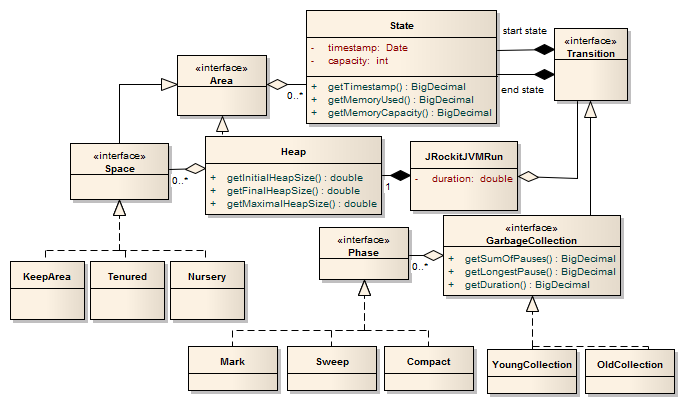
\includegraphics[width=16.5cm]{images/jrockit_extension_domain}
	\caption{Domänenmodell: Garbage Collection (JRockit Implementation)}
\end{figure}
\end{landscape}
Die Daten der Log-Datei repräsentieren einen Lauf einer JVM (\textit{JRockitJVMRun}) bestehend aus einem Heap und den darin enthaltenen Bereichen Keep-Area, Nursery und Tenured Space. Jeder dieser Bereiche hat unterschiedliche Zustände in welchen die verschiedenen Messgrössen gemessen und gespeichert werden. Zustandsübergänge finden durch Transitionen respektive durch eine Garbage Collection statt, es kann sich dabei um Young oder Old Collections handeln. Das starten einer Transition wird durch einen Event ausgelöst (hier im Diagramm nicht ersichtlich), Events werden aufgrund von heuristischen Daten der Lauzeitumgebung geworfen - zum Beispiel wenn die Nursery oder die Old Collection an ihre Speichergrenze gelangen. Der Vollständigkeit halber sind im Diagramm zusätzlich noch die einzelnen Phasen der Garbage Collection definiert, die bei einer Garbage Collection durchlaufen werden.

\subsection{Garbage Collection Logdatei parsen (FRQ-05)}
Die Garbage Collection Logs der JRockit Virtual Machine bestehen aus Einträgen unterschiedlicher Log Module. Diese Ausgaben können selektiv per Kommandozeile aktiviert werden (siehe Abschnit \ref{logmodule}). Für die Garbage Collection Analyse sind nicht alle Einträge interessant, es werden nur die wichtigsten verwendet. Die einzelnen Parser der für die Garbage Collection Logdatei werden auf der Basis von Regular Expressions selber implementiert. Auf die Verwendung eines Parser-Generators wird aus folgenden Gründen verzichtet:
\begin{itemize}
	\item Lightweight: Um Parser-Generatoren zu verwenden, wird in der Regel auch zur Laufzeit eine Bibliothek benötigt. Diese muss mit der Software ausgeliefert werden. Die Implementation von Regulären Ausdrücken beispielsweise ist der Java Laufzeitumgebung sowieso verfügbar.
	\item Proprietär: Parser-Generatoren sind proprietär und die Verwendung dessen bedingt gute Kenntnisse. In der Regel beschreibt man das Format in einer Grammatik.
\end{itemize}

\subsubsection{Parser}
Der Parser für die Logdateien der JRockit Virtual Machine ist nach dem Chain-of-Responsibility Pattern\cite{wiki:chainOfResponsibilityPattern} aufgebaut. Pro Logeintrag (respektive pro Typ) kann ein Parser in die Parser-Kette geschaltet werde. Jeder Parser extrahiert die für ihn wichtigen Informationen und aktualisiert damit das Domänenmodell. Die wichtigsten Einträge des Garbage Collection Logs sind die des Memory Modules und werden vom \textit{MemoryModuleParser} verarbeitet. In zukünftigen Versionen ist die Verarbeitung von Logeinträgen von anderen Log-Modulen denkbar - Einträge des Nursery-, Allocation-Modules, etc. Ablauf und Aufbau des Parsers sind in den folgenden beiden Grafiken ersichtlich:

 \begin{figure}[H]
  	\centering
    	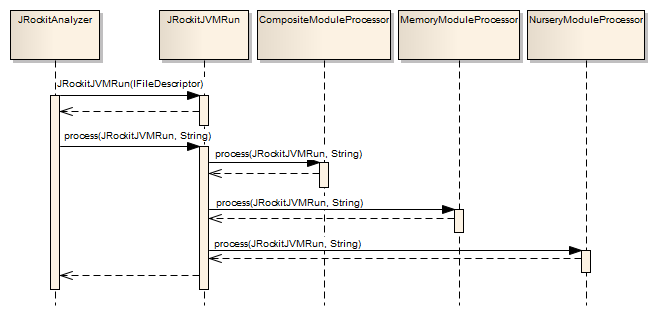
\includegraphics[width=16cm]{images/acitivity_parse_prozess}
        	\caption{Sequenzdiagramm Parsen Logdatei}
\end{figure}
 \begin{figure}[H]
  	\centering
    	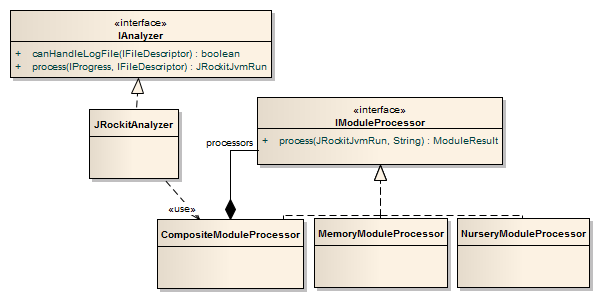
\includegraphics[width=16cm]{images/jrockit_log_processing}
        	\caption{Klassendiagramm Parsen Logdatei}
\end{figure}

\subsubsection{MemoryModuleParser}
Das Parsen innerhalb des \textit{MemoryModuleParser} wird in zwei Schritte aufgeteilt:
\begin{itemize}
\item \textbf{Lexer: }Der einzelne Logeintrag wird durch den Lexer (Tokenizer) in eine Map aus Tokens umgewandelt. Schlüssel für die einzelnen Tokens ist der \textit{TokenType}. Der Lexer wird mittels Regular Expressions implementiert. Die Werte werden mittels Gruppierungs-Funktion\footnote{Mittels Gruppen innerhalb von Regulären Ausdrücken lassen sich einzelne Werte aus einem String extrahieren.} extrahiert. 
\item \textbf{Syntactic Analyzer: }Der syntaktische Analyser verarbeitet die vom Lexer extrahierten Tokens. Er führt zum einen eine semantische Validierung durch und speichert die Werte in strukturierter Form (Domänenmodell).
\end{itemize}

\subsection{Standardauswertung anzeigen (FRQ-06)}
\subsubsection{Anzeige Übersicht Garbage Collection (FRQ-06.1)}\label{standardreport}
Der initiale Tab der Analyseseite zeit eine Zusammenfassung der geöffneten Garbage Collection. Sie wird in verschiedenen Tabellen dargestellt:
\begin{itemize}
	\item Heap Kapazität
	\begin{itemize}
		\item Initiale Kapazität (Nursery, Tenured, Heap)
		\item Maximale Kapazität (Heap)
		\item Speicherbedarf Peak (Heap)
		\item Kapazität Durchschnittlich (Heap)
		\item Speicherbedarf Durchschnittlich (Heap)
	\end{itemize}
	\item Garbage Collection Aktivität (Young und Old Collection)
	\begin{itemize}
		\item Letzter Zyklus
		\item Anzahl Zyklen
		\item Durchschnittlicher Interval in Sekunden
		\item Durchschnittliche Dauer in Sekunden		
	\end{itemize}	
	\item Gesamtstatistik
	\begin{itemize}
		\item Dauer der Messung in Sekunden
		\item Anzahl Garbage Collection Zyklen
		\item Total Zeit der Garbage Collection
		\item Prozentuale Zeit der Garbage Collection
		\item Totale Zeit der Old Garbage Collection Zyklen
		\item Prozentuale Zeit der Old Garbage Collection Zyklen
	\end{itemize}
\end{itemize}

\subsubsection{Chart Anzeige Heap Benutzung (FRQ-06.2)}
Die Heap-Analyse zeigt den Verlauf des benutzten Speichers im Heap über die Zeit auf. Die einzelnen Garbage Collection Zyklen (Young, Old) werden verschiedenfarbig dargestellt.

\subsubsection{Chart Anzeige Dauer Garbage Collection (FRQ-06.3)}
Die Dauer der einzelnen Garbage Collection Zyklen wird über die Zeit aufgezeigt. Die einzelnen Garbage Collection Zyklen (Young, Old) werden verschiedenfarbig dargestellt.


%--------------------------------------------
\section{Qualitätsanforderungen}
\subsection{Testabdeckung (QRQ-S-02)}\label{testing}
Bei Plugin-Projekten wird der Test-Code normalerweise in eigenen Fragment-Projekten abgelegt. Diese Test-Projekte werden allerdings nicht mit dem Feature ausgeliefert, sondern nur während dem Testen verwendet. Der Zugriff auf den Code der Implementation wird gewährleistet, indem aus dem Test-Projekt ein Fragment\footnote{Fragmente haben vollen Zugriff auf ihre Host-Bundles.} gemacht wird.

\section{Eclipse Rich Client Framework}
\subsection{Speicherung des Zustands einer View}\label{memento}
Die Speicherung des Zustands einer View wird von Eclipse unterstützt, indem die Methode \textit{saveState(memento:IMemento)} von \textit{ViewPart} implementiert wird. \textit{IMemento} ist eine Eclipse-Klasse und gleichzeitig die Abstraktion eines Mementos. Memento ist ein Design Pattern und wurde durch die Gang of Four\footnote{Erich Gamma, Richard Helm, Ralph Johnson, John Vlissides} in \cite[S. 283]{gamma1995design} zum ersten Mal definiert. Mementos dienen zur Serialisierung von Objekten und haben den Vorteil, dass auch Klassen aus einem Memento einer anderen Version deserialisiert werden können. Das Eclipse-Framework persistiert die Zustände von Views mittels eines XMLMemento entsprechend im XML-Format ab. Die Deserialisierung erreicht man mit dem Überschreiben der Methode \textit{init(site:IViewSite, memento:IMemento)}.

\subsection{Internationalisierung (QRQ-S-03))}
Die Analysesoftware kann in den Sprachen Deutsch und Englisch gestartet werden. Die gewählte Sprache wird von der Entwicklungsumgebung übernommen\footnote{Die Entwicklungsumgebung übernimmt die Sprache der Java Lauzeitumgebung: Voreinstellung oder Auswahl über Kommandozeile (-nl de). } und kann nicht via ein Menu geändert werden. 
Basierend auf der \textit{Locale}-Klasse der Java Laufzeitumgebung können sprachabhängige Ressourcen geladen werden. Sprachabhängig sind folgende Bereiche:
\begin{itemize}
	\item \textbf{Texte, Labels im Code:} Eclipse stellt zur Externalisierung von Strings einen Wizard zur Verfügung. Die Texte werden in Properties-Dateien extrahiert und beim Starten der Applikation geladen.
	\item \textbf{Texte, Labels in Deskriptoren:} Die sich in den Eclipse-Deskriptoren (plugin.xml und Manifest.MF) befindenden sprachabhängigen Texte wie Organisation, Plugin-Name und -Beschreibung werden ebenfalls in Properties-Dateien extrahiert. Der Ort und Name dieser Dateien ist per Konvention \textit{\textbackslash \$\{plugin\}\textbackslash OSGI-INF\textbackslash I10n\textbackslash bundle\_\$\{lang\}.properties}. Der Inhalt wird vom Eclipse-Framework geladen.
	\item \textbf{Hilfesystem:} Eclipse startet zur Anzeige des auf HTML basierenden Hilfesystems einen Webserver. Die Hilfeseiten können ebenfalls in unterschiedlichen Sprachen definiert werden und werden auf der Basis der gewählten Locale angezeigt.
\end{itemize} 

\subsection{Usability (QRQ-S-04))}
Einige der Funktionalitäten der Analysesoftware wie Beispielsweise das Einlesen und Parsen der Logdateien dauern lange. Der Benutzer benötigt eine Statusinformation. Operationen dieser Art werden mittels des Eclipse \textit{IProgressService} gestartet. Dies hat für die Applikation und den Benutzer folgende Vorteile:
\begin{itemize}
	\item \textbf{Nebenläufigkeit:} Die Applikation startet die Arbeit in einem eigenen nicht-UI Thread\footnote{Einem Thread der nicht für das Zeichnen des Benutzerinterfaces verwendet wird.}, sodass es nicht zu Nebeneffekten wie einem eingefrorenen Bildschirm kommt. Der Benutzer kann die Fortschrittsanzeige minimieren und mit der Applikation weiterarbeiten.
	\item \textbf{Fortschrittsanzeige: } Die Applikation teilt dem Benutzer über eine Anzeige mit, bei welcher Position sich der Prozess befindet und wie viel Arbeit prozentual bereits gemacht wurde.
	\item \textbf{Unterbrechbarkeit: } Der Prozess erkundigt sich periodisch bei der Monitoring-Komponente ob er durch den Benutzer abgebrochen wurde. Sobald dies der Fall wäre, würde er die Arbeit beenden und das bereits Erledigte aufräumen.
\end{itemize}


\subsection{Korrektheit (QRQ-S-05))}



%--------------------------------------------
\section{Infrastruktur}
\subsection{Build-Automatisierung}
Die Automatisierung des Software-Builds ist hinsichtlich der Integration in ein Continuous Integration System wichtig. Zusätzlich entfallen so zeitaufwändige Tasks wie die Paketierung und das Deployment der Applikation.
Als Werkzeug zum automatisierten Build der Software wird Maven Tycho\footnote{Im Bereich der Eclipse Rich Client Entwicklung kann entweder PDE Build, ein auf Apache Ant basiertes Build-System für Eclipse RCP Applikationen\cite{vogelZapfPdeBuild} oder die Maven-Integration Tycho (http://tycho.sonatype.org) verwendet werden.} verwendet.

Tycho ist relativ neu und bringt im Vergleich mit dem PDE Build einige Vorteile mit sich:
\begin{itemize}
	\item Maven folgt dem Prinzip ``Convention over Configuration''\footnote{Das Prinzip ``Convention over Configuration'' hat zur Folge, dass im Wesentlichen nur von den Standardeinstellungen abweichende Werte konfiguriert werden müssen.} - die Konfiguration des Builds wird dadurch wesentlich einfacher.
	\item Maven ist de facto Standard bei den Build-Werkzeugen.
\end{itemize}

\subsection{Versionskontrolle}
Zur Versionsverwaltungssysteme kommen mehrere Werkzeuge in Frage. Git\footnote{http://git-scm.com} ist ein verteiltes Sourcecode Management System und ist konzeptionell und hinsichtlich Benutzerfreundlichkeit besser als Subversion und CVS\footnote{Git kann offline verwendet werden, das Verschieben von Verzeichnissen führt nicht zu Problemen, etc.}. Auf der Plattform Github\footnote{http://github.com} kann man öffentliche Projekte gratis ``hosten''.


\subsection{Continous Integration}
Continuous Integration Systeme dienen zur Steigerung der Softwarequalität. Sie machen dies in der Regel, indem sie alle Tests und den Gesamtbuild der Software periodisch - üblich ist jede Stunde - durchführen. Für die Analysesoftware gibt es bei der Evaluation einige Grundvoraussetzungen:
\begin{itemize}
	\item \textbf{Buildwerkzeug Maven:} Das System muss Maven als Build- und Automatisierungswerkzeug unterstützen.
	\item \textbf{Git Versionskontrolle:} Der Quelltext der Applikation muss via Git vom Sourcecode Repository ausgecheckt werden können.
	\item \textbf{Freie Lizenz:} Die Software muss mindestens frei verfügbar sein oder open-source.
\end{itemize}
In den letzten Jahren hat sich Hudson\footnote{Vor kurzem haben sich einige Entwickler von Hudson aufgrund von Streitigkeiten mit Oracle dazu entschieden, die Software weiter unter dem Namen Jenkins zu entwickeln.} in vielen Projekten durchgesetzt. Hudson ist eine open-source Continuous Integration Software die gegenüber anderen Systemen einige Vorteile mit sich bringt:
\begin{itemize}
\item Hudson ist open-source.
\item Hudson ist sehr einfach zu installieren und administrieren.
\item Hudson basiert auf einem Plugin-System und ist aufgrund dessen erweiterbar. Es gibt Plugins für die Integration von Maven-Projekten und den Zugriff auf Git Repositories.
\end{itemize}



\subsection{Issue Tracker}
Als Issue Tracker wird Jira verwendet. Es handelt sich dabei um eine kostenpflichtige aber relativ günstige Software für das Issue-Tracking.


